\chapter{Effects of bursting and senescence}

There are many different phenomena that could have an effect on noise. Most of the models that have been based on assumptions and have made fits of the data obatined with fluorescent proteins according to those assumptions. Nevertheless, we will see in this chapter that noise coming from different mechanisms could have the same general behaviors, making it difficult to predict characteristics of the systems according to their noise.

We will use the Fluctuation-Dissipation theorem as we used it on chapter \ref{ch:fdt} to analyize the effects of bursting (the synthesis of several molecules per creation event) and senescence (the degradation of molecules over many steps) on noise.

This chapter is based on the work done by J. M. Pedraza and J. Paulsson in \cite{pedraza08}.

Transcription and translation does not occur necessarily as single step Poisson processes. Due to the complexity of gene regulation, their statistics may not be so simple. There are cases where many copies of mRNA are created in short periods of time (bursting). Also, promoters may take several steps to become active (gestation), and mRNAs and proteins to degrade (senescence). Figure \ref{bur-examples} shows some examples of bursting and senescence.

\begin{figure}[H]
  \centering
  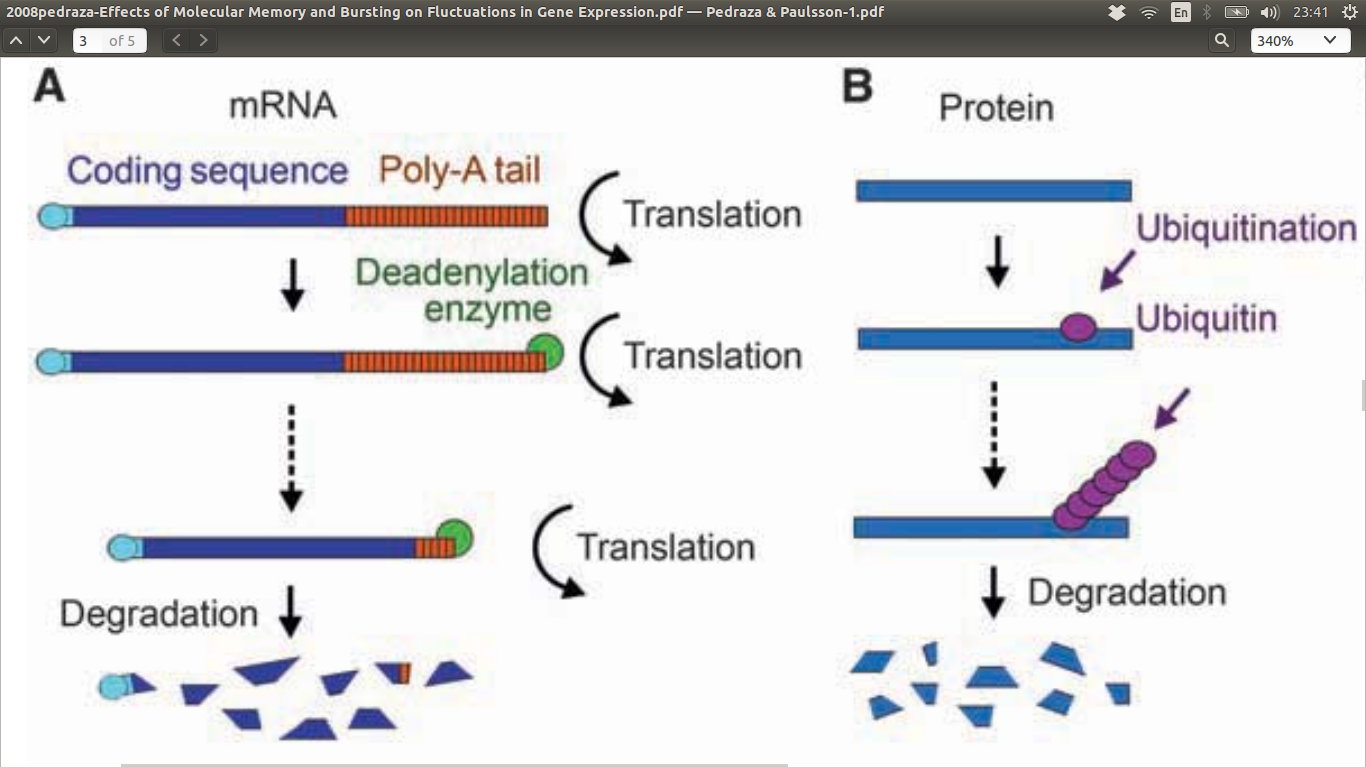
\includegraphics[width=8cm]{bur-examples}
  \caption[Examples of bursting and senescence in gene expression]{\label{fig:bur-examples} Examples of bursting and senescene in gene expression.(left) Example of a promoter where many transcription factors bind in successive steps taking a random time $T$. When the complex is bound to the promoter, A random number $b$ of transcription events occur in a time much shorter than $T$.(right) Senescene in eukaryotic mRNAs occurs when their poly(A) tail\footnotemark is sequentially removed before the part that is translated is degraded. Translation can occur while the poly(A) tail is removed. Taken from \cite{pedraza08}.}
\end{figure}

\footnote{The poly(A) tail is an additional stretch of mRNA that is not part of the protein coding sequence. It is important for the processing of mRNA.}

\section{mRNA bursts}
Let the mRNA be produced with bursts of random size $b$, the degradation and protein creation is done one at a time with exponential waiting times (single-step Poisson processes). In this case the only modification with respect to the ``standard model'' (eqs. \eqref{eq:mas-simple_det_1} and \eqref{eq:mas-simple_det_2}) is the $D_{11}$ term of the matrix $\mathbf{D}$, which by definition is

\begin{equation}
  \label{eq:mrnab1}
  D_{11}=\frac{1}{\langle n_1\rangle^2}\sum_k(s_1^k)^2r_k(\mathbf{n}).
\end{equation}

All the possible $k$ reactions include all the creation bursts and the reaction of degradation, which has rate $\nicefrac{\langle n_1 \rangle}{\tau_1}$ and $s_1=-1$, therefore

\begin{equation}
  \label{eq:mrnab2}
  \sum_k(s_1^k)^2r_k = \frac{\langle n_1 \rangle}{\tau_1} + \sum_{k'}(s_1^{k'})^2r_{k'}.
\end{equation}

Where now the index $k'$ runs over all the synthesis reactions only. We can rewrite the second term as \footnote{For simplicity, we used the dummy index $k$ on the following calculations, keeping in mind that it only runs along the synthesis reactions.}

\begin{equation*}
  \sum_k(s_1^k)^2r_k=\sum_kr_k\sum_k\left(\frac{r_k}{\sum_kr_k}\right)(s_1^k)^2,
\end{equation*}

where the sum over the term in parentheses results in $1$. This term can be interpreted as the probability that the upcoming reaction turns out to be the $k^{\text{th}}$ one. Writing it as $\rho_k$ this yields

\begin{equation*}
  \sum_k(s_1^k)^2r_k=\sum_kr_k\sum_k\rho_k(s_1^k)^2,
\end{equation*}

but $s_1^k$ is the burst size for the $k^{\text{th}}$ synthesis reaction. Therefore the inner sum of the previous equation is actually an average over all the possible burst sizes, hence

\begin{equation}
  \label{eq:mrnab4}
  \sum_k(s_1^k)^2r_k=\sum_kr_k\langle b^2 \rangle=\left(\langle b\rangle^2+\sigma_b^2\right)\sum_kr_k,
\end{equation}

and using a similar trick we get

\begin{equation*}
  \begin{split}
    \sum_kr_k&=\sum_kr_ks_1^k\frac{\sum_kr_k}{\sum_kr_ks_1^k}=\sum_kr_ks_1^k\left(\sum_k\left(\frac{r_k}{\sum_kr_k}\right)s_1^k\right)^{-1}\\
    &=\sum_kr_ks_1^k\left(\sum_k\rho_ks_1^k\right)^{-1}=\frac{1}{\langle b\rangle}\sum_kr_ks_1^k.
  \end{split}
\end{equation*}

Assuming the system is in steady state, all the synthesis rates equal the degradation ones. Therefore

\begin{equation*}
  \sum_kr_ks_1^k = \frac{\langle n_1\rangle}{\tau_1},
\end{equation*}

obtaining

\begin{equation*}
   \sum_kr_k = \frac{\langle n_1\rangle}{\langle b\rangle\tau_1}.
\end{equation*}

Replacing this on eq. \eqref{eq:mrnab4}, and then on eq. \eqref{eq:mrnab2} and \eqref{eq:mrnab1} we get

\begin{equation}
  \label{eq:d11}
  D_{11}=\frac{1}{\langle n_1\rangle^2}\left(\frac{\langle n_1\rangle}{\tau_1}+\frac{\langle n_1\rangle}{\langle b\rangle\tau_1}\left(\langle b\rangle^2+\sigma_b^2\right)\right) = \frac{1}{\tau_1\langle n_1\rangle}\left( 1+ \langle b\rangle\left(1+\frac{\sigma_b^2}{\langle b\rangle^2}\right)\right)
\end{equation}

The matrices then become

\begin{equation*}
  \mathbf{D} = 
  \begin{pmatrix}
    D_{11} & 0 \\
    0 & \frac{2}{\tau_2\langle n_2\rangle}
  \end{pmatrix}, \quad
  \mathbf{M} =
  \begin{pmatrix}
    \frac{1}{\tau_1} & 0 \\
    -\frac{1}{\tau_2} & \frac{1}{\tau_2}
  \end{pmatrix}.
\end{equation*}

With $D_{11}$ given by eq. \eqref{eq:d11} And solving the linear system $\mathbf{M}\mathbf{\eta} + \mathbf{\eta M}^T+\mathbf{D}=0$ (see sec. \ref{sec:log_gain}), we obtain the following expression for the noise in the proteins

\begin{equation}
  \boxed{\eta_{22}=\frac{1}{\langle n_2\rangle} + \frac{1}{\langle n_1\rangle} \frac{\tau_1}{\tau_1 + \tau_2} \frac{\langle b\rangle\left(1+\nicefrac{\sigma_b^2}{\langle b\rangle^2}\right)+1}{2}}.
\end{equation}

\todo[inline]{TODO: Analysis of the equations, independence on details of the distribution}

\section{Arbitrary distribution of creation times}

Suppose a creation event happened at $t=0$, and let $f(t)$ be the probability density function of a creation event happening at time $t$ (meaning a time $t$ after the last event), i.e. $P(t\in[T,T+dt])=f(T)dt$. According to that, the following properties are satisfied

\begin{equation*}
P(n=0|t=T) = P(t>T) = 1 - P(t<T) = 1 - F(T)
\end{equation*}

where $n$ stands for the number of creation events and $F$ is the cumulative distribution function associated to $f(t)$. Also, for one creation event to have happened before time $t=T$, there must be a creation on a time $t_1$ such that $0<t_1<T$ and no creation events on the remaining ($T-t_1$) time. This leads to the following equation

\begin{equation*}
  \begin{split}
    P(n=1|t=T) &= \int_0^TP(t=t_1)P(t>T-t_1)\mathrm{d}t_1 \\
    &= \int_0^Tf(t_1)(1-F(T-t_1))\mathrm{d}t_1=f\ast (1-F)|_T,
  \end{split}
\end{equation*}

where the asterisk denotes the convolution product. Following a similar argument, we obtain for an arbitrary number of events

\begin{equation}
  \label{eq:nconvs}
  \begin{split}
    P(n=N|t=T) &= f\ast P(n=N-1|t)|_T = f\ast f\ast P(n=N-2|t)|_T \\
    &= \cdots = \underbrace{f\ast\cdots\ast f}_{n \text{ times}}\ast P(n=0,t)|_T = \underbrace{f\ast\cdots\ast f}_{n \text{ times}}\ast (1-F)|_T.
  \end{split}
\end{equation}

Since the convolutions are difficult to deal with, we will use the Laplace transform and solve on Laplace space. The property that $\mathcal{L}(f\ast g) = \hat{f}\cdot\hat{g}$, where $\hat{f}\coloneqq\mathcal{L}(f)$ will make the problem much simpler.

Aplying $\mathcal{L}$ to eq. \eqref{eq:nconvs} we get

\begin{equation*}
  \hat{P}(n,s) = \hat{f}^n(s)\mathcal{L}(1-F)(s).
\end{equation*}

It can be easily shown that $\hat{F} = \hat{f}/s$ and $\hat{1} = 1/s$ yielding

\begin{equation}
  \label{eq:lapP}
  \hat{P}(n,s) = \frac{1}{s}\hat{f}^n(s)(1-\hat{f}(s)).
\end{equation}

To find the moments and the noise, we will use the moment generating function, as defined on \eqref{def:mom_gen}. It will be denoted as $G(z,s)$.

\begin{equation}
  \label{eq:lapG}
  \hat{G}(z,s) = \sum_{n=0}^{\infty}z^n\hat{P}(n,s) = \frac{1}{s}(1-\hat{f}(s))\sum_{n=0}^{\infty}(z\hat{f})^n=\frac{1-\hat{f}(s)}{s(1-z\hat{f}(s))}.
\end{equation}

Where the geometric series convereges in this case because $\hat{f}(s)\leq1$ and we will evaluate $z$ at $1$. The first and second derivatives of $G$ in Laplace space are given by

\begin{equation}
  \label{eq:lapavn}
  \langle\hat{n}\rangle(s) = \left.\frac{\partial\hat{G}(z,s)}{\partial z}\right|_1 = \frac{\hat{f}(s)}{s(1-\hat{f}(s))}.
\end{equation}

\begin{equation}
  \label{eq:lapvarn}
  \langle\hat{n}(\hat{n}-1)\rangle(s) = \left.\frac{\partial^2\hat{G}(z,s)}{\partial z^2}\right|_1 = \frac{2}{s}\left(\frac{\hat{f}(s)}{1-\hat{f}(s)}\right)^2.
\end{equation}

It could also be proven that

\begin{equation}
  \label{eq:lapfprop}
  \hat{f}(0) = 1, \quad \left.\frac{\mathrm{d}\hat{f}(s)}{\mathrm{d}s}\right|_0=-\langle t\rangle,\quad \left.\frac{\mathrm{d}^2\hat{f}(s)}{\mathrm{d}s^2}\right|_0=\langle t^2\rangle.
\end{equation}

Therefore applying the inverse Laplace transform to eqs. \eqref{eq:lapavn} and \eqref{eq:lapvarn}, and using properties \eqref{eq:lapfprop} we could obtain the moments. 

\begin{equation}
  \langle n\rangle(t) = \mathcal{L}^{-1}(\langle\hat{n}\rangle(s))=\frac{1}{2i\pi}\oint e^{st}\frac{\hat{f}(s)}{s(1-\hat{f}(s))}\mathrm{d}s
\end{equation}

The integral can be solved by residues. Since $\hat{f}(0)=1$, there is a pole of order $2$ in $s=0$. To find the residues of a pole $c$ of order $m$ of the function $f$, the residue is given by

\begin{equation}
  \label{eq:residues}
  \text{Res}_c(f)=\frac{1}{(m-1)!}\lim_{z\to c}\frac{\mathrm{d}^{m-1}}{\mathrm{d}z^{m-1}}((z-c)^mf(z)).
\end{equation}

Then

\begin{equation*}
  \begin{split}
    \langle n\rangle(t)&=\text{Res}_0\frac{e^{st}}{s}\frac{\hat{f}(s)}{1-\hat{f}(s)}=\lim_{s\to0}\frac{\mathrm{d}}{\mathrm{d}s}\frac{se^{st}\hat{f}(s)}{1-\hat{f}(s)}\\
    & = \lim_{s\to0}\frac{e^{st}}{(\hat{f}(s)-1)^2}\left[(1+st)(\hat{f}(s)-1)\hat{f}(s) + s\hat{f}'(s)\right].
  \end{split}
\end{equation*}

To find the limit we have to apply L'Hospital rule twice, after some algebra it yields

\begin{equation}
  \label{eq:aven}
  \langle n\rangle(t)=\frac{\hat{f}''(0)}{2(\hat{f}'(0))^2}-\frac{t}{\hat{f}'(0)}-1=\frac{t}{\langle t\rangle}+\left(\frac{\langle t^2\rangle}{2\langle t\rangle^2}-1\right).
\end{equation}

Now inverting eq. \eqref{eq:lapvarn} we obtain

\begin{equation*}
  \begin{split}
    \langle n(n-1)\rangle(t)&=\frac{1}{2i\pi}\oint e^{st}\frac{2}{s}\left(\frac{\hat{f}(s)}{1-\hat{f}(s)}\right)^2\mathrm{d}s=\text{Res}_0\frac{2}{s}\left(\frac{\hat{f}(s)}{1-\hat{f}(s)}\right)^2\\
&=\lim_{s\to0}\frac{\mathrm{d}^2}{\mathrm{d}s^2}e^{st}\left(\frac{s\hat{f}(s)}{1-\hat{f}(s)}\right)^2
  \end{split}
\end{equation*}

Where we used eq. \eqref{eq:residues} to find the residue of a pole of order $3$. After doing the necessary algebra and the L'Hospital rule three times we get

\begin{equation*}
  \langle n(n-1)\rangle(t)=\frac{t^2}{\langle t\rangle^2}+\frac{4t}{\langle t\rangle}\left(\frac{\langle t^2\rangle}{2\langle t\rangle^2}-1\right)+2\left(1-\frac{\langle t^2\rangle}{\langle t\rangle^2}+\frac{3\langle t^2\rangle^2}{4\langle t\rangle^4}+\frac{\langle t^3\rangle}{3\langle t\rangle^3}\right)
\end{equation*}

And combining with eq. \eqref{eq:aven} we obtain the variance

\begin{equation}
  \label{eq:stdn}
  \sigma_n^2(t) = \frac{t}{\langle t\rangle}\left(\frac{\langle t^2\rangle}{\langle t\rangle^2}-1\right)+\left(-\frac{\langle t^2\rangle}{2\langle t\rangle^2} + \frac{5\langle t^2\rangle^2}{4\langle t\rangle^4}-\frac{2\langle t^3\rangle}{3\langle t\rangle^3}\right).
\end{equation}

\todo[inline]{Analysis, (compare with the exponential case) and explain why we ignore the other part}

Ignoring the second terms in parentheses in eqs. \ref{eq:aven} and \ref{eq:stdn} we get

\begin{align}
  \langle n\rangle &= \frac{t}{\langle t\rangle}, \label{eq:avena} \\
  \sigma_n^2 &= \frac{t}{\langle t\rangle}\left(\frac{\langle t^2\rangle}{\langle t\rangle^2}-1\right). \label{eq:stdna}
\end{align}

Rearranging eq. \eqref{eq:stdna} and using eq. \eqref{eq:avena} we get

\begin{equation*}
  \sigma_n^2 = \frac{t}{\langle t\rangle}\left(\frac{\langle t^2\rangle - \langle t\rangle^2}{\langle t\rangle^2}\right) = \frac{t}{\langle t\rangle}\eta_t^2 = \langle n\rangle\eta_t^2.
\end{equation*}

Hence

\begin{equation}
  \label{eq:noisen1}
  \eta_n^2=\frac{1}{\langle n\rangle}\eta_t^2.
\end{equation}

Now we will include the effect of bursts of creation. Let $n$ be the number of creation events on a given time interval (meaning the number of bursts, not the total number of molecules created), $b_i$ be burst size for the $i^{\text{th}}$ events. Both $n$ and $b_i$ are random variables, and each $b_i$ follows the same probability distribution. Consider the random variable

\begin{equation}
  \label{eq:xtotal}
  x\coloneqq\sum_{i=0}^nb_i
\end{equation}

representing the total number of molecules created on the given time interval. (It is a sum of a random number of random variables). We will denote the probability mass function of $x$ as $P_x(x)$.

We will use the properties of the characteristic function $\phi(s)$ and find the moments using its properties (see sec. \ref{sec:con-charac_func}). From its definition

\begin{equation*}
  \phi(s) \coloneqq \langle e^{xs}\rangle_x = \sum_{a=0}^\infty e^{xs}P_x(x=a).
\end{equation*}

Using the total probability theorem, we can write it as

\begin{equation}
  \label{eq:charac1}
  \begin{split}
    \phi(s) &= \sum_{a=0}^\infty e^{xs}\sum_{n=0}^\infty P_x(x=a|n)P(n) = \sum_{n=0}^\infty\left(\sum_{a=0}^\infty e^{xs}P_x(x=a|n)\right)P(n)\\ 
&= \sum_{n=0}^\infty \langle e^{xs}\rangle_{x|n} P(n)
  \end{split}
\end{equation}

Where $\langle\quad\rangle_x$ denotes average with respect to the distribution of $x$. Using eq. \eqref{eq:xtotal} we get for $\langle e^{xs}\rangle_{x|n}$

\begin{equation*}
  \langle e^{xs}\rangle_{x|n} = \langle e^{s\sum_{i=0}^nb_i} \rangle_b = \langle \prod_{i=0}^ne^{sb_i}\rangle_b,
\end{equation*}

Notice that the average is now taken with respect to the distribution of burst sizes (denoted by $\langle\quad \rangle_b$) since we wrote the function in terms of that variable. Assuming independence of the burst sizes we get

\begin{equation*}
  \langle e^{xs}\rangle_{x|n} =  \prod_{i=0}^n\langle e^{sb_i}\rangle_b,
\end{equation*}

and since all the $b_i$s follow the same distribution, the product is in fact independent of $i$, yielding

\begin{equation*}
  \langle e^{xs}\rangle_{x|n} = \prod_{i=0}^n\langle e^{sb}\rangle_b = \langle e^{sb}\rangle_b^n
\end{equation*}.

Replacing this result in eq. \eqref{eq:charac1} we obtain

\begin{equation*}
  \phi(s) = \sum_{n=0}^\infty \langle e^{sb}\rangle_b^n P(n) = \left\langle\langle e^{sb}\rangle_b^n\right\rangle_n
\end{equation*}

Where $\langle\quad\rangle_n$ denotes average with respect to the distribution of events $P_n$.

We proceed to obtain the moments, using the properties of the characteristic function (eqs. \eqref{eq:con-char_2} - \eqref{eq:con-char_2})

\begin{equation}
  \label{eq:avex}
  \langle x\rangle = \left.\frac{\mathrm{d}\phi(s)}{\mathrm{d}s}\right|_0 = \left.\frac{\mathrm{d}}{\mathrm{d}s}\left\langle\langle e^{bs}\rangle_b^n\right\rangle_n\right|_0 = \left.\left\langle n\langle e^{bs}\rangle_b^{n-1}\langle b e^{bs}\rangle_b\right\rangle_n\right|_0 = \left\langle n\langle b\rangle_b\right\rangle_n = \langle n\rangle_n\langle b\rangle_b,
\end{equation}

which is intuitive: the average number of molecules produced is the average number of bursts times the average burst size. For the second moment we have

\begin{equation*}
  \begin{split}
    \langle x^2\rangle &= \left.\frac{\mathrm{d^2}\phi(s)}{\mathrm{d}s^2}\right|_0 = \left.\frac{\mathrm{d}\phi(s)}{\mathrm{d}s}\left\langle n\langle e^{bs}\rangle_b^{n-1}\langle b e^{bs}\rangle_b\right\rangle_n\right|_0\\
  &= \left.\left\langle n(n-1)\langle e^{bs}\rangle^{n-2}_b\langle be^{bs}\rangle^2_b+n\langle e^{bs}\rangle^{n-1}_b\langle b^2e^{bs}\rangle_b\right\rangle_n\right|_0\\
  &=\langle n^2\rangle_n\langle b\rangle_b^2-\langle n\rangle_n\langle b\rangle_b^2+\langle n\rangle_n\langle b^2\rangle_b.
  \end{split}
\end{equation*}

Using the previous result with eq. \eqref{eq:avex} to find the variance we differentiate twice

\begin{equation*}
  \begin{split}
    \sigma_x^2 &= \langle n^2\rangle_n\langle b\rangle_b^2-\langle n\rangle_n\langle b\rangle_b^2+\langle n\rangle_n\langle b^2\rangle_b - \langle n\rangle_n^2\langle b\rangle_b^2\\
    &=\langle b\rangle_b^2\left(\langle n^2\rangle_n-\langle n\rangle^2_n\right) + \langle n\rangle_n\left(\langle b^2\rangle_b-\langle b\rangle_b^2\right)\\
    &=\langle b\rangle_b^2\sigma_n^2 + \langle n\rangle_n\sigma_b^2.
  \end{split}
\end{equation*}

Dividing by $\langle x\rangle^2=\langle n\rangle_n^2\langle b\rangle_b^2$,

\begin{equation*}
  \eta_x^2=\frac{\sigma_n^2}{\langle n\rangle_n^2} + \frac{\sigma_b^2}{\langle n\rangle_n\langle b\rangle_b^2} = \eta_n^2+\frac{1}{\langle n\rangle_n}\eta_b^2.
\end{equation*}

Using eq. \ref{eq:noisen1} we obtain

\begin{equation}
  \label{eq:noisex}
  \eta_x^2=\frac{1}{\langle n\rangle}\left(\eta_t^2+\eta_n^2\right)=\frac{\langle b\rangle\left(\eta_t^2+\eta_n^2\right)}{\langle x\rangle},
\end{equation}

where

\begin{equation}
  \langle x\rangle = \langle b\rangle\frac{t}{\langle t\rangle}.
\end{equation}

This result holds for a pure birth process.

\section{Decay of molecules}

We include the effects of decay of molecules considering a binomial partitioning during cell division. Let $P_\text{Dr}(l|m)$ be the probability of finding $l$ molecules in volume fraction $r$ given that there are $m$ molecules before division.

Assuming that each molecule segregates independently, and that the probability of arriving at a volume is proportional to it we obtain a binomial distribution

\begin{equation}
  P_\text{Dr}(l|m) = {m\choose l}r^l(1-r)^{m-l}.
\end{equation}

Let $P_\text{Br}(m)$ and $P_\text{Ar}(m)$ be the probabilities of having $m$ molecules before and after division, respectively, for a fixed volume fraction $r$. We have then

\begin{equation}
  P_\text{Ar}(l) = \sum_{m=0}^\infty P_\text{Dr}(l|m)P_\text{Br}(m) = \sum_{m=0}^\infty {m\choose l}r^l(1-r)^{m-l}P_\text{Br}(m).
\end{equation}

Multiplying by $z^l$ and summing we get the moment generating function $G_\text{Ar}(z)$

\begin{equation}
  \label{eq:binomG}
  \begin{split}
    G_\text{Ar}(z) &= \sum_{l=0}^\infty z^l\sum_{m=0}^\infty {m\choose l}r^l(1-r)^{m-l}P_\text{Br}(m)\\
    &= \sum_{m=0}^\infty\left(\sum_{l=0}^\infty (zr)^l(1-r)^{m-l}\right)P_\text{Br}(m).\\
    &= \sum_{m=0}^\infty(zr+1-r)^{m}P_\text{Br}(m),
  \end{split}
\end{equation}

where we used the binomial expansion formula on the last step.

The number of molecules of at the end of a growth stage (following $P_\text{Br}$) equals the number of molecules at the beginning (following $P_\text{Ar}$) plus the number of molecules created during the cycle (following $P_{x,\tau} \coloneqq P_x|_{t=\tau}$). Assuming both random variables as independent and recalling that the probability mass function of the sum of random variables is the convolution of the individual PMFs we have

\begin{equation*}
  P_\text{Br}(m) = P_\text{Ar}\ast P_{x,\tau}(m)
\end{equation*}

Therefore,

\begin{equation}
  G_\text{Br}(z) = G_\text{Ar}(z)G_{x,\tau}(z).
\end{equation}

Finding the moments by using the properties of $G$ and the previous equation we obtain

\begin{equation*}
  \langle n\rangle_\text{Br} = \left.\frac{\partial G_\text{Br}(z)}{\partial z}\right|_1 = G_\text{Ar}(1)\left.\frac{\partial G_{x,\tau}(z)}{\partial z}\right|_1 + \left.\frac{\partial G_\text{Ar}(z)}{\partial z}\right|_1G_{x,\tau}(1) = \langle m\rangle_{x,\tau} + \langle m\rangle_\text{Ar},
\end{equation*}

from eq. \ref{eq:binomG} 

\begin{equation*}
  \begin{split}
  \left.\frac{\partial G_\text{Ar}(z)}{\partial z}\right|_1 &= \langle m\rangle_\text{Ar} = \left.\frac{\partial}{\partial z} \sum_{m=0}^\infty(zr+1-r)^mP_\text{Br}(m)\right|_1\\
&= \left.\sum_{m=0}^\infty m(zr+1-1)^{m-1}rP_\text{Br}(m)\right|_1\\
&= r\sum_{m=0}^\infty mP_\text{Br}(m) = r\langle m\rangle_\text{Br}
  \end{split}
\end{equation*}
  
Therefore

\begin{equation}
  \label{eq:aveBrAr}
  \langle m\rangle_\text{Br} = \frac{1}{1-r}\langle m\rangle_{x,\tau}\quad\quad \langle m\rangle_\text{Ar} = r\langle n\rangle_\text{Br} = \frac{r}{1-r}\langle m\rangle_{x,\tau}.
\end{equation}

The variances are obtained by taking the second derivative

\begin{equation}
  \label{eq:2Br}
  \begin{split}
    \langle m(m-1)\rangle_\text{Br} &= \left.\frac{\partial^2 G_\text{Br}(z)}{\partial z^2}\right|_1\\
    &=G_\text{Ar}(1)\left.\frac{\partial^2 G_{x,\tau}(z)}{\partial z^2}\right|_1 + \left.\frac{\partial^2 G_\text{Ar}(z)}{\partial z^2}\right|_1G_{x,\tau}(1) + 2\left.\frac{\partial G_\text{Ar}(z)}{\partial z}\right|_1\left.\frac{\partial G_{x,\tau}(z)}{\partial z^2}\right|_1\\
    &=\langle m(m-1)\rangle_{x,\tau}+\langle m(m-1)\rangle_\text{Ar}+2\langle m\rangle_{x,\tau}\langle m\rangle_\text{Ar}.
  \end{split}
\end{equation}

but from eq. \ref{eq:binomG}

\begin{equation}
  \label{eq:2Ar}
  \begin{split}
    \langle m(m-1)\rangle_\text{Ar} &= \left.\frac{\partial^2}{\partial z^2}\sum_{m=0}^\infty(zr+1-r)^mP_\text{Br}(n)\right|_1\\
    &= \left.\sum_{m=0}^\infty m(m-1)(zr+1-r)^{m-2}r^2P_\text{Br}(n)\right|_1 = r^2\langle n(n-1)\rangle_\text{Br}.
  \end{split}
\end{equation}

For any random variable $x$, we can write $\langle x(x-1)\rangle = \sigma_x^2 - \langle x\rangle + \langle x\rangle^2$. Using this on eqs. \ref{eq:2Br} and \ref{eq:2Ar} we get

\begin{equation*}
  \begin{split}
  \sigma^2_\text{Br}- \langle m\rangle_\text{Br} + \langle m\rangle^2_\text{Br} &= \left( \sigma^2_{x,\tau} - \langle m\rangle_{x,\tau} + \langle m\rangle_{x,\tau}^2\right)\\
&+ 2\left(r\langle m\rangle_\text{Br}\right)\left[(1-r)\langle m\rangle_\text{Br}\right]+r^2\left(\sigma^2_\text{Br}- \langle m\rangle_\text{Br} + \langle m\rangle^2_\text{Br}\right)
  \end{split}
\end{equation*}

After some algebra we obtain

\begin{equation}
  \label{eq:sigmaBr}
  \sigma^2_\text{Br} = \frac{1}{1-r^2}\sigma^2_{x,\tau}+\frac{r}{1+r}\langle m\rangle_\text{Br}
\end{equation}

Dividing by $\langle m\rangle_\text{Br}^2$ and using eq. \ref{eq:aveBrAr} we get

\begin{equation}
  \begin{split}
    \eta_\text{Br}^2 &= \frac{1}{1-r^2}\sigma_{x,\tau}^2\frac{(1-r)^2}{\langle m\rangle_{x,\tau}^2} + \frac{r}{1+r}\langle m\rangle_\text{Br}\\
    & = \frac{1-r}{1+r}\eta_{x,\tau}^2+\frac{r}{1+r}\frac{1}{\langle n\rangle_\text{Br}}
  \end{split}
\end{equation}

Also, from eqs. \ref{eq:2Ar} and \ref{eq:sigmaBr} we get

\begin{equation}
  \begin{split}
    \sigma^2_\text{Ar} - \langle m\rangle_\text{Ar} + \langle m\rangle_\text{Ar}^2 &= r^2\left(\sigma^2_\text{Br}- \langle m\rangle_\text{Br} + \langle m\rangle^2_\text{Br}\right)\\
  &=r^2\left(\frac{1}{1-r^2}\sigma^2_{x,\tau}+\frac{r}{1+r}\langle m\rangle_\text{Br}\right)-r^2\langle m\rangle_\text{Br} + r^2\langle m\rangle^2_\text{Br}
  \end{split}
\end{equation}

Using eq. \ref{eq:aveBrAr} and after a little algebra we get

\begin{equation}
  \sigma^2_\text{Ar} = \frac{r^2}{1-r^2}\sigma^2_{x,\tau}+\frac{1}{1+r}\langle m\rangle_\text{Ar},
\end{equation}

hence, dividing by $\langle m\rangle_\text{Ar}^2$ and using eq. \ref{eq:aveBrAr} we get

\begin{equation}
  \begin{split}
    \eta^2_\text{Ar} &= \frac{r^2}{1-r^2}\sigma^2_{x,\tau}\left(\frac{1-r}{r\langle m\rangle_{x,\tau}}\right)^2+\frac{1}{1+r}\frac{1}{\langle m\rangle_\text{Ar}}\\
    &=\frac{1-r}{1+r}\eta^2_{x,\tau}+\frac{1}{1+r}\frac{1}{\langle m\rangle_\text{Ar}}.
  \end{split}
\end{equation}

\todo[inline]{Understand the intermediate steps here and complete}

\begin{equation}
  \boxed{\eta^2 = \frac{\langle b\rangle\left(\eta^2_t + \eta^2_b\right)+1}{2\langle n\rangle}}
\end{equation}

\todo[inline]{Complete and analyze here also}

\section{Senescence of mRNA}

Suppose that mRNAs are created at a constant rate $\lambda_1$ and that they senesce through a sequence of $N$ steps labeled as $X_1,X_2,\dotsc,X_N$. Thus, the states and their transitions are

\begin{equation}
  \text{Transcription} \rightarrow X_1 \rightarrow X_2 \rightarrow \dots \rightarrow X_N \rightarrow \text{Degradation}
\end{equation}

The number of mRNA molecules in each step is labeled as $x_i$ for $1\leq i\leq N$. Also, assume that the rates of transcription $\beta_1$ per mRNA between the states are the same. The possible transtions in the state space are thus

\begin{equation}
  \begin{split}
    x_1&\xrightarrow{\lambda_1}x_1+1\\
    \{x_i,x_{i+1}\}&\xrightarrow{\beta_1x_i} \{x_i-1,x_{i+1}+1\},\quad \text{for}\quad1\leq i\leq N-1\\
    x_N&\xrightarrow{\beta_1x_N} x_N-1
  \end{split}
\end{equation}

Where the first line denotes transcription, the second denotes transitions between states and the third stands for degradation. Now, denote as $x_{N+1}$ the number of proteins in a cell and suppose that independently of the current state of the mRNA molecules, they are translated with the same rate $\lambda_2$ per mRNA. Also, denoting the degradation rate per protein as $\beta_2$ the possible transitions for the proteins are

\begin{equation}
  \begin{split}
    x_{N+1} &\xrightarrow{\lambda_2\sum_{i=1}^Nx_i} x_{N+1}+1,\\
    x_{N+1} &\xrightarrow{\beta_2x_{N+1}}x_{N+1}-1.
  \end{split}
\end{equation}

Then, the average dynamics are

\begin{equation}
  \begin{split}
    \dot{\langle x_1\rangle} &= \lambda-1 -\beta_1\langle x_1\rangle,\\
    \dot{\langle x_{i+1}\rangle} &= \beta_1\left(\langle x_i\rangle - \langle x_{i+1}\rangle\right)\quad\text{for}\quad 1\leq i\leq N,\\
    \dot{\langle x_{N+1}\rangle} &= \lambda_2\sum_{i=1}^N\langle x_i\rangle-\beta_2\langle x_{N+1}\rangle.
  \end{split}
\end{equation}

At steady state we get

\begin{equation}
  \begin{split}
    \langle x_1\rangle &= \frac{\lambda_1}{\beta_1},\\
    \langle x_{i+1}\rangle &= \langle x_i\rangle\quad\text{for}\quad 1\leq i\leq N-1,\\
    \langle x_{N+1}\rangle &= \frac{\lambda_2}{\beta_2}\sum_{i=1}^N\langle x_i\rangle.
  \end{split}
\end{equation}

Therefore,

\begin{equation}
  \langle x_i\rangle = \lambda_1\tau_1\quad\text{for}\quad 1\leq i\leq N,
\end{equation}

where $\tau_1 \coloneqq \nicefrac{1}{\beta_1}$.

Denoting the total mRNA as $m$, then $m=\sum_{i=1}^Nx_i$ and taking the average

\todo[inline]{Complete this}
